\section{Democracy Index}

There are plenty of sources for measuring democracy levels. Our World in Data mainly uses six: Varieties of Democracy (V-Dem), the Lexical Index of Electoral Democracy (LIED) by Skaaning et al. (2015), Freedom House's (FH) Freedom in the World index, the Bertelsmann Transformation Index (BTI) by the Bertelsmann Foundation, the Economist Intelligence Unit's (EIU) Democracy Index, and Polity by the Center for Systemic Peace \cite{herre_democracy_2025}. 

Out of the six mentioned datasets, only V-Dem and LIED have data spanning between 1946 and 2025. However, V-Dem offers more granularity and is generally considered a more complete and robust dataset. It is the best choice if we are interested in both large and small differences in varieties of democracy far into the past, or if we want to use country experts to measure characteristics of political systems that are difficult to observe. These experts are anonymous and are primarily academics or members of the media and civil society. They are also often nationals or residents of the country they assess; therefore, they know its political system well and can evaluate aspects that are difficult to observe. V-Dem's own team of researchers supplements these expert evaluations \cite{herre_varieties_2025}.

\subsection{Varieties of Democracy Dataset}

All data is available for download at \url{https://v-dem.net/data/the-v-dem-dataset/} or can be accessed directly as an R package.

V-Dem distinguishes between \textit{indicators}—lower-level data that is often not normalized—and \textit{indices}, which aggregate indicators and are normalized on a scale between zero and one.

There are four datasets: \textit{Coder-Level}, with raw data and 273 indicators intended for the experts; \textit{CD Country-Date}, with day-to-day granularity, 531 indicators, and 95 aggregated indices; \textit{CY Country-Year}, with year-level granularity, 5 indices, 93 sub-indices, and 179 indicators; and lastly, \textit{CY Full + Others}, with year-level granularity, 531 indicators, 251 indices, and 62 external indicators. 

I must use the \textit{CD Country-Date} dataset (version 16, released in March 2026) since, to keep track of Italian governments, year-level granularity is not enough. This is evident from Figure \ref{fig:italyPms}: half of Italy's governments lasted less than a year.

\begin{figure}[h]
  \centering
  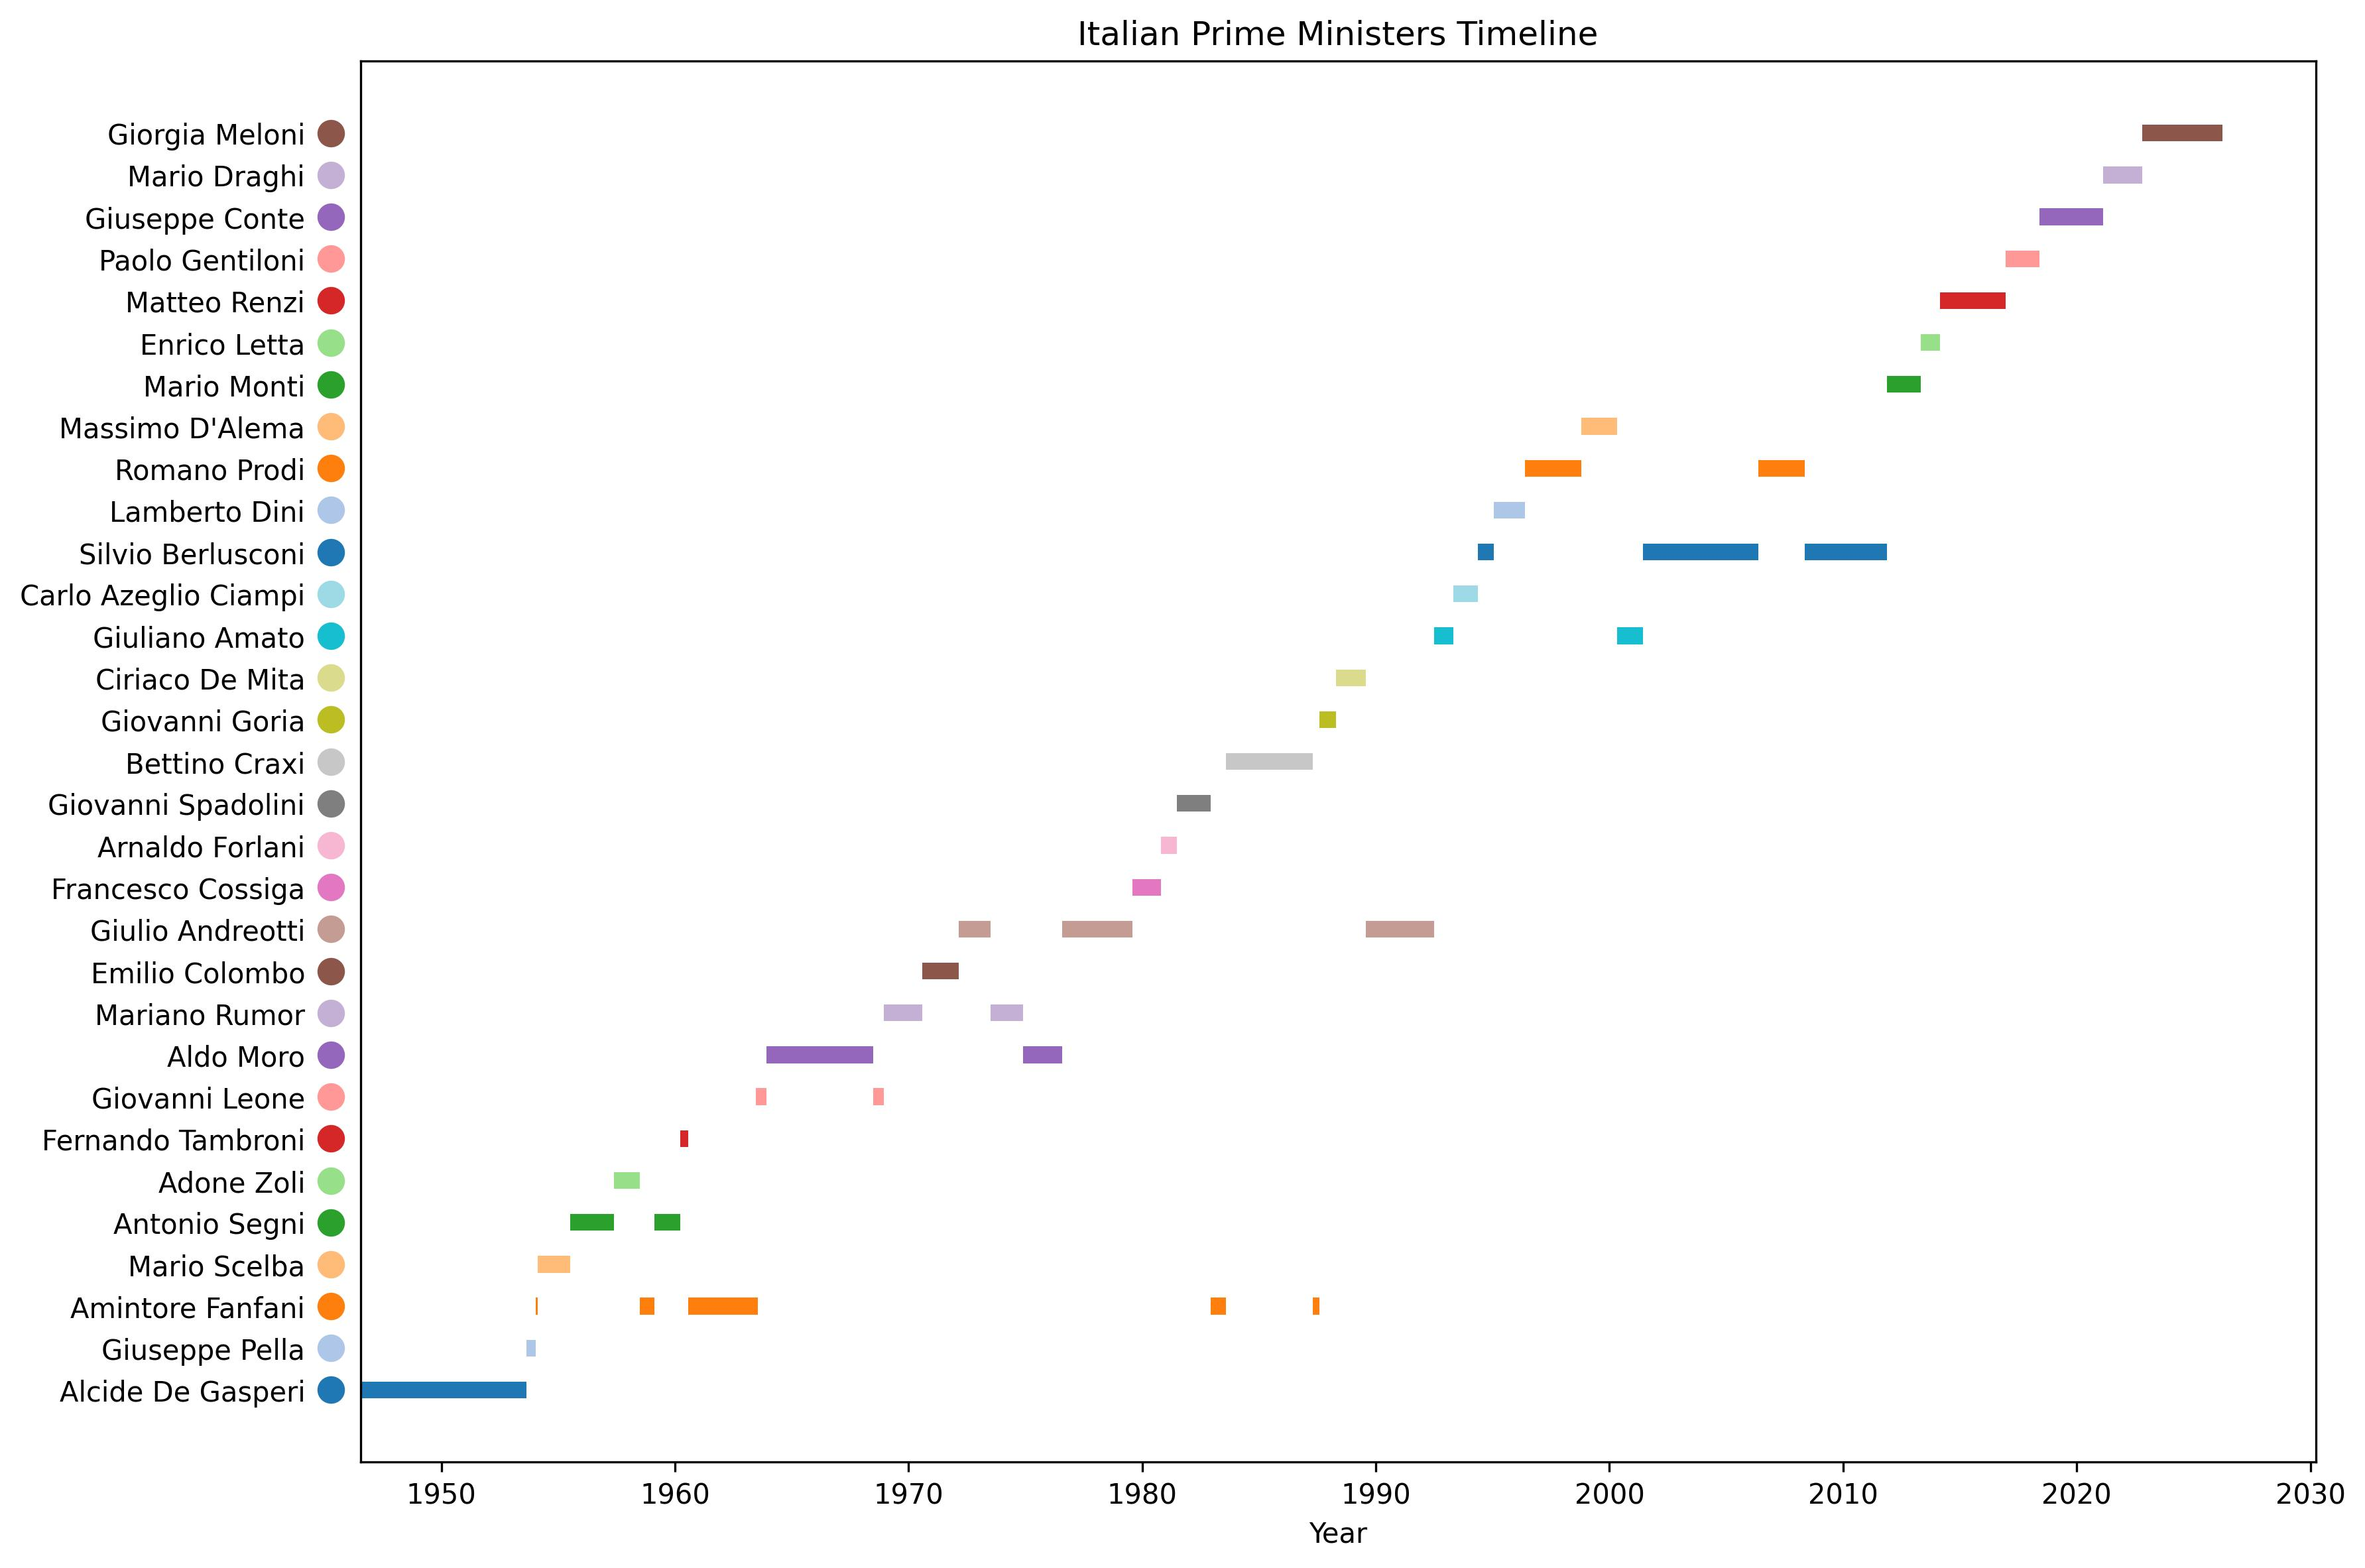
\includegraphics[width=.7\linewidth]{images/italian_prime_ministers.jpg}
  \caption{Italian Prime Ministers for each Italian Republic, from the first (1946) to the latest (2025).}
  \Description{All Italian Prime Ministers shown by their days in charge.}
  \label{fig:italyPms}
\end{figure}

The dataset covers Italy (ID 82) between 1861 and 2025, France (ID 76) between 1789 and 2025, and the U.S. (ID 20) between 1789 and 2025.

Useful identifiers include: \texttt{country\_id}, unique for each country; \texttt{country\_text\_id}, ISO 3166-1 alpha-2 country codes (e.g., \textit{IT}, \textit{FR}); \texttt{historical\_date}, in \textit{YYYY-MM-DD} format, used for election-date-specific variables (all other variables use January 1st); and \texttt{gapstart} and \texttt{gapend}, representing time periods where no data is available.

\textbf{Democracy Indices} are the highest-level indices, each normalized to a scale between zero and one unless otherwise specified: \texttt{v2x\_polyarchy}, the \textit{electoral} democracy index (aggregates \texttt{v2x\_elecoff}, \texttt{v2xel\_frefair}, \texttt{v2x\_frassoc\_thick}, \texttt{v2x\_suffr}, \texttt{v2x\_freexp\_altinf}); \texttt{v2x\_libdem}, the \textit{liberal} democracy index (aggregates \texttt{v2x\_polyarchy}, \texttt{v2x\_liberal}); \texttt{v2x\_partipdem}, the \textit{participatory} democracy index (aggregates \texttt{v2x\_polyarchy}, \texttt{v2x\_partip}); \texttt{v2x\_delibdem}, the \textit{deliberative} democracy index focusing on process, respectful dialogue, and the common good (aggregates \texttt{v2x\_polyarchy}, \texttt{v2xdl\_delib}); and \texttt{v2x\_egaldem}, the \textit{egalitarian} democracy index considering social status, inequalities, and resource distribution (aggregates \texttt{v2x\_polyarchy}, \texttt{v2x\_egal}).

\textbf{Components of Democracy Indices} consist of second-level indices and subcomponents: \texttt{v2x\_freexp\_altinf}, freedom of expression and alternative information (aggregates \textit{v2mecenefm}, \textit{v2meharjrn}, \textit{v2meslfcen}, \textit{v2xcl\_disc}, \textit{v2clacfree}, \textit{v2mebias}, \textit{v2mecrit}, \textit{v2merange}); \texttt{v2x\_frassoc\_thick}, freedom of association for parties and civil society organizations (aggregates \textit{v2psparban}, \textit{v2psbars}, \textit{v2psoppaut}, \textit{v2elmulpar}, \textit{v2cseeorgs}, \textit{v2csreprss}, \texttt{v2x\_elecreg}); \texttt{v2x\_suffr}, the percentage of adult suffrage (aggregates \textit{v2elsuffrage}); \texttt{v2xel\_frefair}, the quality of free and fair elections (aggregates \textit{v2elembaut}, \textit{v2elembcap}, \textit{v2elrgstry}, \textit{v2elvotbuy}, \textit{v2elirreg}, \textit{v2elintim}, \textit{v2elpeace}, \textit{v2elfrfair}, \texttt{v2x\_elecreg}); \texttt{v2xcl\_rol}, rule of law, transparency, and fair enforcement (aggregates \textit{v2clrspct}, \textit{v2cltrnslw}, \textit{v2cltort}, \textit{v2clkill}, \textit{v2clrelig}, \textit{v2clfmove}, \texttt{v2xcl\_dmove}, \texttt{v2xcl\_slave}, \texttt{v2xcl\_acjst}, \texttt{v2xcl\_prpty}); \texttt{v2x\_jucon}, executive law compliance and judiciary independence (aggregates \textit{v2exrescon}, \textit{v2jucomp}, \textit{v2juhccomp}, \textit{v2juhcind}, \textit{v2juncind}); \texttt{v2xlg\_legcon}, executive external scrutiny (aggregates \textit{v2lgqstexp}, \textit{v2lgotovst}, \textit{v2lginvstp}, \textit{v2lgoppart}); \texttt{v2x\_partip}, individual participation (aggregates \texttt{v2x\_cspart}, \texttt{v2xdd\_dd}, \texttt{v2xel\_locelec}, \texttt{v2xel\_regelec}); \texttt{v2x\_cspart}, participation in associations like labor unions or NGOs (aggregates \textit{v2pscnslnl}, \textit{v2cscnsult}, \textit{v2csprtcpt}, \textit{v2csgender}); \texttt{v2xdd\_dd}, the direct vote index for referendums and ballots (aggregates \textit{v2ddlexci} through \textit{v2ddthreci}); \texttt{v2xel\_regelec} and \texttt{v2xel\_locelec}, regional and local government elections; \texttt{v2xeg\_eqprotec}, equal rights across social groups; \texttt{v2xeg\_eqaccess}, equality of accessing power; and \texttt{v2xeg\_eqdr}, equality of resource distribution (aggregates \textit{v2dlencmps}, \textit{v2dlunivl}, \textit{v2peedueq}, \textit{v2pehealth}).


